\documentclass[12pt]{scrartcl}
\usepackage[utf8]{inputenc}
\usepackage{microtype}
\usepackage{amsmath}
\usepackage{amsfonts}
\usepackage{amssymb}
\usepackage{graphicx}
\usepackage{xcolor}
\usepackage{booktabs}
\usepackage[colorlinks]{hyperref}
\usepackage[numbers]{natbib}
\usepackage{geometry}
\usepackage{xurl}

\geometry{margin=1in}

\definecolor{linkcolor}{HTML}{800006}
\definecolor{citecolor}{HTML}{2E7E2A}
\definecolor{filecolor}{HTML}{131877}
\definecolor{urlcolor}{HTML}{8A0087}
\definecolor{menucolor}{HTML}{727500}
\definecolor{runcolor}{HTML}{137776}

\hypersetup{
	linkcolor=linkcolor,
	citecolor=citecolor,
	filecolor=filecolor,
	urlcolor=urlcolor,
	menucolor=menucolor,
	runcolor=runcolor,
}

\title{A data-driven assessment of Continuum of Care effectiveness in addressing homelessness among older adults (65+) in California}
\author{Im\`ene R. Goumiri \and Amanda L. Muyskens}
\date{Real Good AI \\[1em] July 2025}

\begin{document}

\maketitle

\begin{abstract}
Evaluating the effectiveness of California's Continuums of Care (CoCs) in addressing homelessness among older adults is confounded by external factors like population size and housing costs, which make direct comparisons misleading. This study utilizes a Random Forest model to control for these variables and provide a more equitable assessment of CoC performance. Our model confirms that total population is the primary predictor of homeless counts, but also reveals that geographic location is a surprisingly strong factor, likely acting as a proxy for unmeasured socioeconomic conditions. By normalizing for population and housing costs, our counterfactual analysis identifies CoCs that are performing significantly better or worse than expected. Notably, several large urban CoCs, including those in Los Angeles County, demonstrate strong relative performance despite facing the greatest raw numbers, while regions like San Diego/Imperial and the northern coast show potential underperformance. These findings suggest a need to shift policy focus from raw counts towards a nuanced, data-driven evaluation to identify best practices and target interventions more effectively.
\end{abstract}

%\clearpage

\section{Introduction}

This report presents a data-driven assessment of Continuum of Care (CoC) effectiveness in addressing homelessness among adults aged 65 and over in California. The analysis uses publicly available data to model factors associated with homelessness counts at the CoC level, with the goal of identifying which CoCs perform differently than expected given their demographic and geographic context.

\subsection{Background: homelessness in california}

California has a disproportionate share of the United States' homeless population. In 2024, the state accounted for 24\% of the nation's total, despite having only 12\% of its population~\cite{ppic2025homelessness}. This crisis has worsened in recent years, with the number of people experiencing homelessness increasing by 6\% between 2020 and 2022~\cite{calich2025hdis}. This growth is largely attributed to systemic factors, particularly a severe housing affordability crisis where housing costs have outpaced supply and incomes~\cite{ppic2025homelessness, huduser2019market}. While California has invested significant funds into programs aimed at reducing homelessness, a statewide audit noted a lack of information to assess the effectiveness of these programs, highlighting a need for evidence-based evaluation~\cite{ppic2025homelessness}.

Within this context, older adults (65+) are a growing and vulnerable demographic. The number of adults 65 and older accessing homelessness services in California increased by over 166\% from 2017 to 2022~\cite{terner2023older}. A significant portion of this group experiences homelessness for the first time later in life, often due to economic shocks rather than chronic individual issues~\cite{terner2023older, cmaj2024late}. This demographic also faces compounded challenges, including high rates of disabling conditions and significant racial disparities, with Black, Indigenous, and Pacific Islander individuals being heavily overrepresented~\cite{terner2023older, calbudgetcenter2025rise}. These factors suggest that effective interventions must address both economic precarity and the specific needs of this aging population.

\subsection{Research objectives}

This study evaluates the performance of California's 44 Continuums of Care (CoCs), the regional bodies responsible for coordinating local homelessness responses~\cite{huduser2000coc}. CoC performance is known to be heterogeneous, influenced by factors both internal (e.g., funding, governance) and external (e.g., housing markets, population size) to the organization~\cite{preprints2025coc}.

The primary objective is to evaluate CoC performance by comparing observed homelessness counts against a statistically derived expectation. To achieve this, we first develop predictive models based on population and geographic factors to establish a ``prediction set" for each CoC—a range of expected homelessness counts given its context. By comparing a CoC's actual count to its prediction set, we can identify which are performing better or worse than anticipated. This study employs a dual-modeling strategy: a Random Forest model, valued for its high predictive accuracy and ability to capture complex, non-linear interactions, and an Analysis of Covariance (ANCOVA) model, which offers a more traditional, interpretable framework for assessing the significance of each factor while controlling for others. This comparative approach allows for a more robust evaluation of CoC effectiveness.

This work builds on other data-driven analyses of homelessness, such as HUD's studies of market factors~\cite{huduser2019market}, the California Policy Lab's predictive prevention models~\cite{capolicylab2025hpu}, and UCSF's large-scale surveys~\cite{ucsf2025studies}. Our contribution is the specific focus on the 65+ age group at the sub-state level in California and the use of a comparative modeling approach to identify relative CoC performance under controlled conditions. The goal is to produce interpretable results that can inform policy and resource allocation.

\section{Data and methods}

The analysis relies on an integrated dataset constructed from several public sources. The unit of analysis is the Continuum of Care (CoC). The key variables are the number of homeless individuals categorized by year and by age group, the total population, the average housing cost, and geographic attributes.

\subsection{Dependent variable: homelessness counts}

The outcome variable is the count of individuals experiencing homelessness in each CoC.

\paragraph{Source:} Data was obtained from the ``Homelessness Count By Age" dataset on the California Open Data portal~\cite{caopendatahomelessness}. This dataset is compiled from the Homelessness Data Integration System (HDIS), which aggregates information from service providers across all 44 California CoCs~\cite{calich2025hdis}. The data covers the period from 2017 to 2023.

\paragraph{Limitations:} The HDIS data primarily captures individuals who interact with the formal service system. It may undercount the total homeless population, particularly unsheltered individuals who do not access services. Furthermore, data from certain providers (e.g., for domestic violence victims) is excluded by law~\cite{calich2025hdis}. This means that a higher count in a CoC could reflect a larger homeless population or more effective outreach at bringing people into the service system. This ambiguity is a key consideration in the interpretation of the results.

\subsection{Independent variables: year, age group, population, geography, and housing costs}

\subsubsection{Year and age group}
The HDIS data is grouped by year, from 2017 to 2023, and by the following age groups: under 18, 18-24, 25-34, 35-44, 45-54, 55-64, 65+, unknown, and invalid.
We have chosen to discard the unknown and invalid categories to minimize noise.

\subsubsection{Population estimates}
To contextualize homelessness counts, population data for each CoC was required.

\paragraph{Source:} Population figures were sourced from the U.S. Census Bureau, including American Community Survey (ACS) estimates and Decennial Census data~\cite{censusgov}.

\paragraph{Processing:} A key step was to align population data, typically reported at the county or city level, with CoC boundaries. CoC and county geographies are not congruent; a CoC may comprise multiple counties, or a single large county may be divided into several CoCs. To resolve this, GIS shapefiles for both CoCs~\cite{hudexchange2024gis} and counties~\cite{caopendatacountyb} were used.
\begin{itemize}
    \item For CoCs that align with one or more full counties, the populations of the constituent counties were summed.
    \item For CoCs that are subdivisions of a larger county (e.g., the four CoCs within Los Angeles County), city-level population data from the Census Bureau was used to approximate the population of each CoC by summing the populations of the cities within its boundaries.
\end{itemize}

Population estimates are shown in the left panel of \autoref{fig:maps}.

\begin{figure}[htbp]
    \centering
    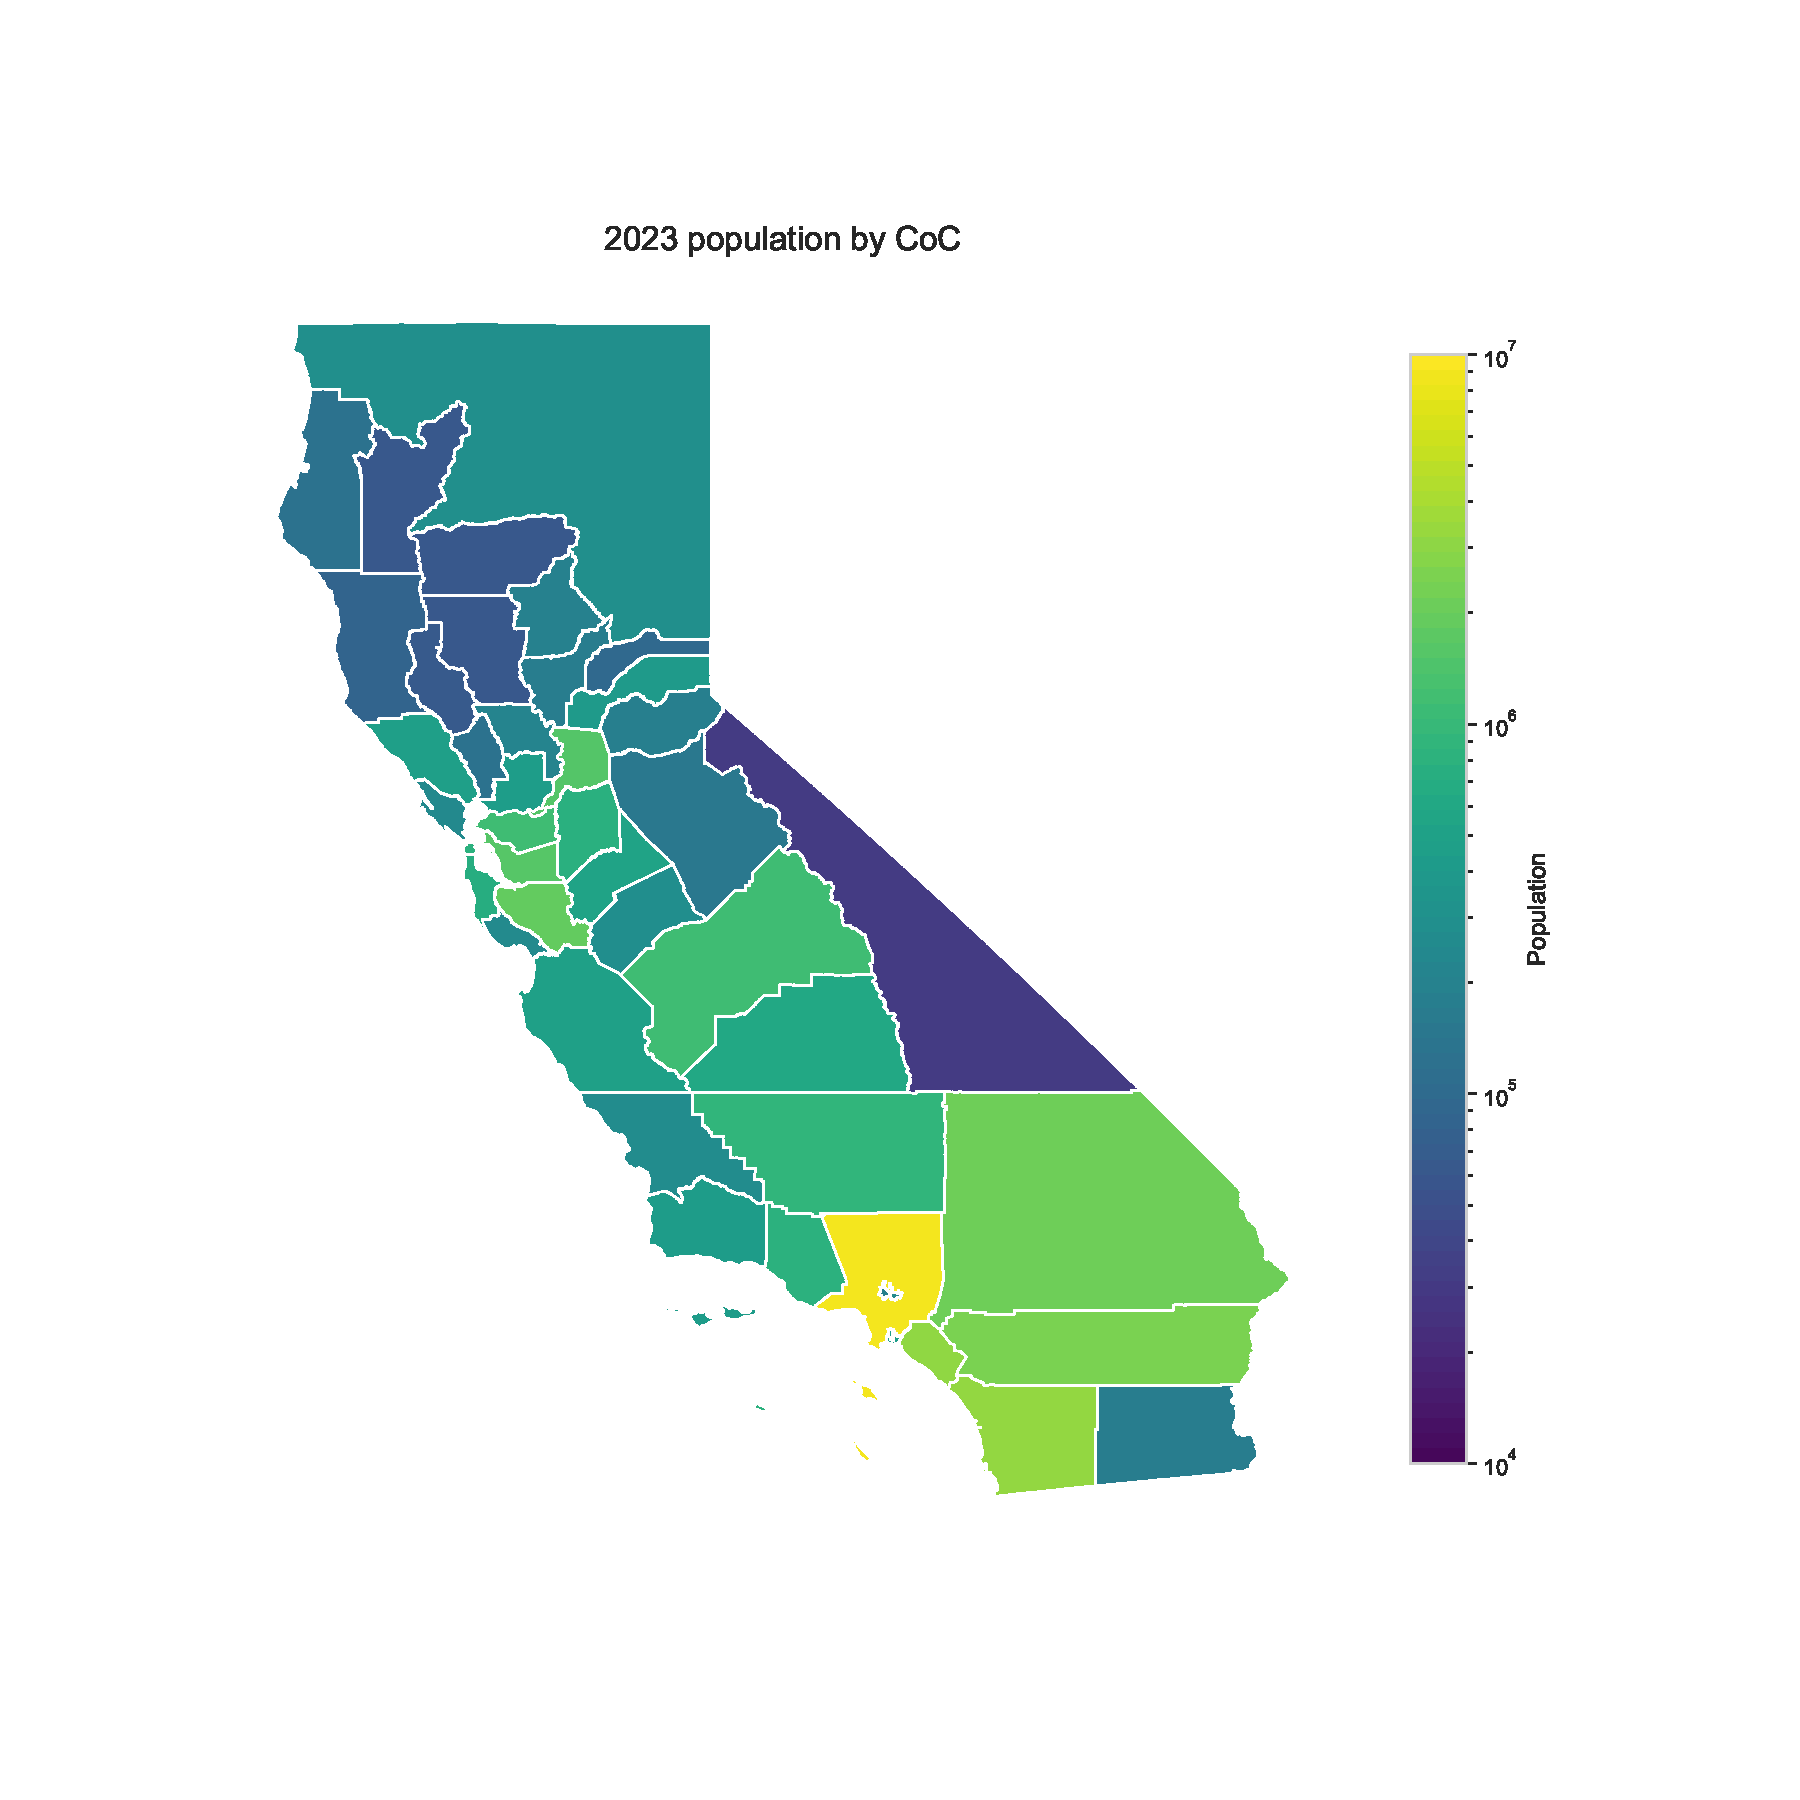
\includegraphics[width=0.5\linewidth, trim={1.5in 1.5in 1.5in 1in}, clip]{figures/maps/population}%
    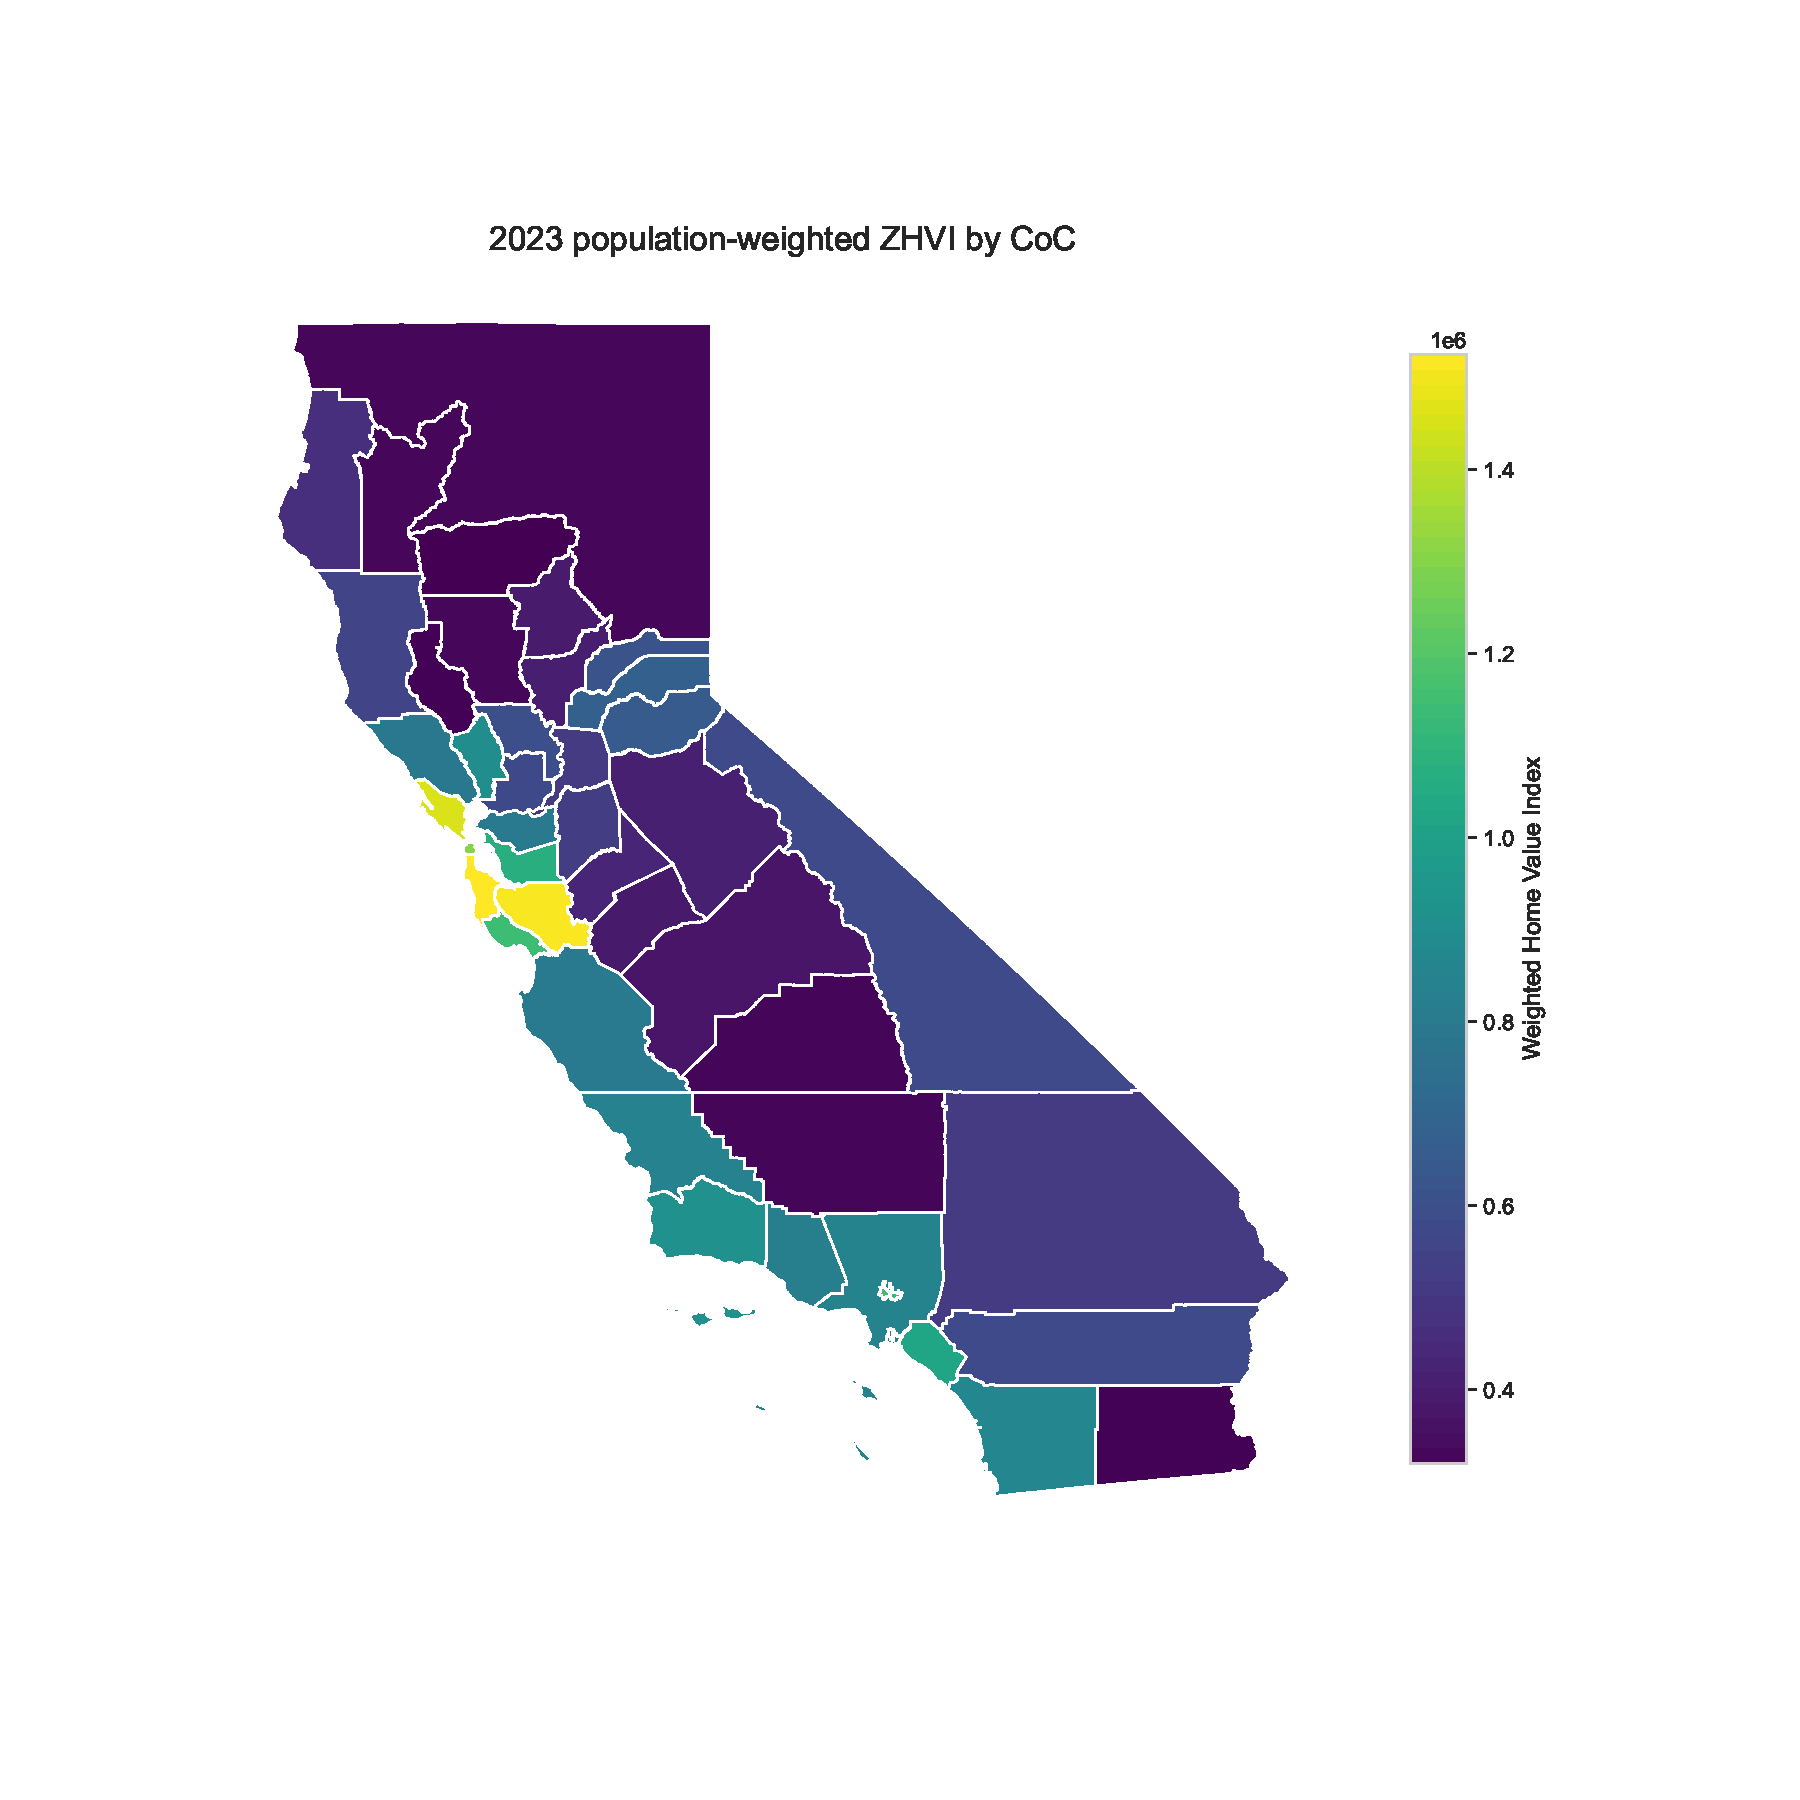
\includegraphics[width=0.5\linewidth, trim={1.5in 1.5in 1.5in 1in}, clip]{figures/maps/housing_cost}
    \caption{
        \label{fig:maps}
        Total population (log scale, left) and housing cost (ZHVI, right) in California CoCs in 2023.
    }
\end{figure}

\subsubsection{Housing cost data}
To account for the influence of local housing markets, a key economic driver of homelessness, housing cost data was incorporated.

\paragraph{Source:} The Zillow Home Value Index (ZHVI) for all homes (including single-family residences, condos, and co-ops), using the smoothed, seasonally adjusted time series, was used as the primary measure of housing cost~\cite{zillow2025data}.

\paragraph{Processing:} The ZHVI data is available at both the county and city level. Similar to the population data, these values were aggregated to the CoC level. For CoCs composed of whole counties, a population-weighted average of the county-level ZHVI was calculated. For CoCs within a single county, a similar weighted average was computed using city-level ZHVI and population data. This ensures that the housing cost metric for each CoC accurately reflects its specific geographic and demographic composition.

Housing cost is represented in the right panel of \autoref{fig:maps}.

\subsubsection{Geographical features}
To account for spatial effects, two geographic features were constructed for each CoC: a geographic center and a list of adjacent CoCs.

\paragraph{Source:} CoC boundary shapefiles were obtained from the HUD Exchange~\cite{hudexchange2024gis}.

\paragraph{Processing:}
\begin{itemize}
    \item \textbf{Centroids:} The geometric centroid (latitude and longitude) of each CoC's polygon shapefile was calculated to provide a single geographic point representing its location~\cite{mygeodesycentroid}.
    \item \textbf{Adjacency:} A CoC adjacency graph was constructed by identifying which CoCs share a common border, based on a spatial analysis of their shapefiles. Then the population-weighted average of the homelessness counts were calculated to form a variable called \emph{spatial lag}. This allows the model to account for potential spillover effects or shared regional characteristics between neighboring CoCs.
\end{itemize}

%%%%%%%%%%%%%%%%%%%%%%%%

\section{Analysis}

\subsection{Modeling approach}
The analysis employs two distinct modeling techniques to provide a comprehensive assessment. A Random Forest model is used for its strength in capturing complex, non-linear relationships and interactions between variables without strong distributional assumptions. This is complemented by an Analysis of Covariance (ANCOVA) model, which provides a more traditional linear framework to assess the impact of specific factors while controlling for covariates like population size~\cite{field2013discovering}. Using both models allows for a more robust interpretation: Random Forest identifies the most influential predictors overall, while ANCOVA offers clear insights into the direction and magnitude of linear relationships.

\subsection{Feature selection and specification}
To mitigate the potential for non-linearity and heteroscedasticity, all continuous features for the ANCOVA model were first normalized to a $[0,1]$ scale. Following normalization, a variety of transformations---including exponential, square root, and square ($x^2$)---were assessed. A modified logarithm transformation, $\log(x+1)$, was employed to prevent infinite results given the range of the normalized features. Beyond these individual transformations, we also considered cross-term interactions between features (both transformed and untransformed). The random forest model, being inherently robust to non-linear relationships, was trained on the untransformed data. Final model selection was based on a combination of superior performance metrics, such as a lower RMSE and a higher $R^2$, and for the ANCOVA, a better adherence to the assumptions of linear regression.
 
\subsection{Model interpretation}
Insights were drawn by synthesizing the results from both models. For the Random Forest, feature importance was calculated using both Gini importance and permutation-based methods to produce a robust ranking of the predictors' influence on homelessness counts. For the ANCOVA model, the analysis focused on the estimated coefficients to determine the direction, magnitude, and statistical significance of each variable's linear relationship with the outcome, after controlling for other factors.

Comparing the findings from both models provides a more nuanced understanding. For example, a variable with high importance in the Random Forest but a non-significant coefficient in the ANCOVA model may suggest a non-linear effect or an effect that is mediated through complex interactions with other variables.

\subsection{Evaluating CoC performance}
To compare CoC performance on a more equitable basis, we use a ``prediction set" approach to control for external factors that are largely outside a CoC's control (e.g., population size, regional economic conditions). This method involves the following steps:
\begin{enumerate}
    \item For each CoC, a standardized data profile is created by replacing its actual values for key external variables with a common baseline (e.g., the statewide average). CoC-specific attributes remain unchanged.
    \item The trained models are then used to generate a predicted homelessness count for each CoC based on this standardized profile.
    \item The resulting predictions allow for a ranking of CoCs based on their expected performance under similar external conditions.
\end{enumerate}
This counterfactual analysis helps to isolate the potential impact of local strategies and operations from the influence of broader demographic and economic contexts, providing a more insightful basis for evaluating relative effectiveness.

%%%%%%%%%%%%%%%%%%%

\section{Results and discussion}

\subsection{Model performance and key drivers of homelessness}

The Random Forest model demonstrated a strong ability to predict homelessness counts. The best-performing models achieved a Root Mean Squared Error (RMSE) of approximately 300. Given that homeless counts range from just a few individuals in rural CoCs to many thousands in large urban ones, this level of error indicates that the model is a reliable tool for this analysis.
% Visually, the model's predictions in \autoref{fig:prediction_set} effectively replicate the geographic distribution of homelessness seen in the observed data (\autoref{fig:observed}), particularly the high concentration in Los Angeles county.

To understand the factors driving these predictions, we analyzed the importance of each input feature. Both Gini-based and permutation-based importance measures consistently identified the total population as the most significant predictor by a large margin (\autoref{fig:feature_importance}). This is expected, as a larger population naturally presents a larger pool of individuals at risk of homelessness. Following population, the spatial lag and housing cost were the next most important factors, while geographic coordinates played a smaller, but still relevant, role.

\begin{figure}[htbp]
    \centering
    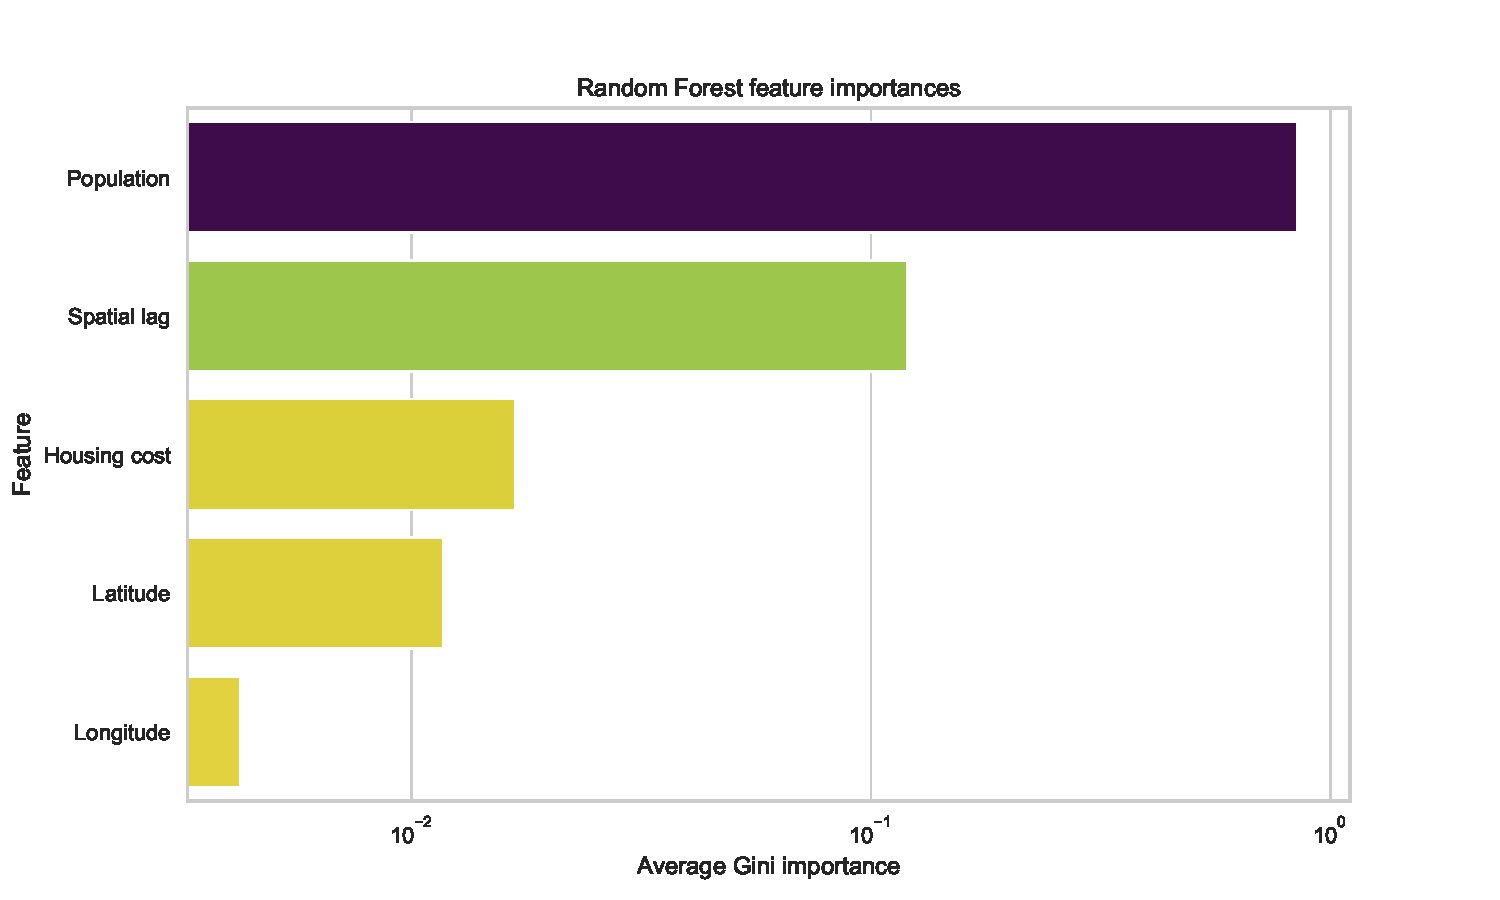
\includegraphics[width=0.5\linewidth]{figures/rf_gini}%
    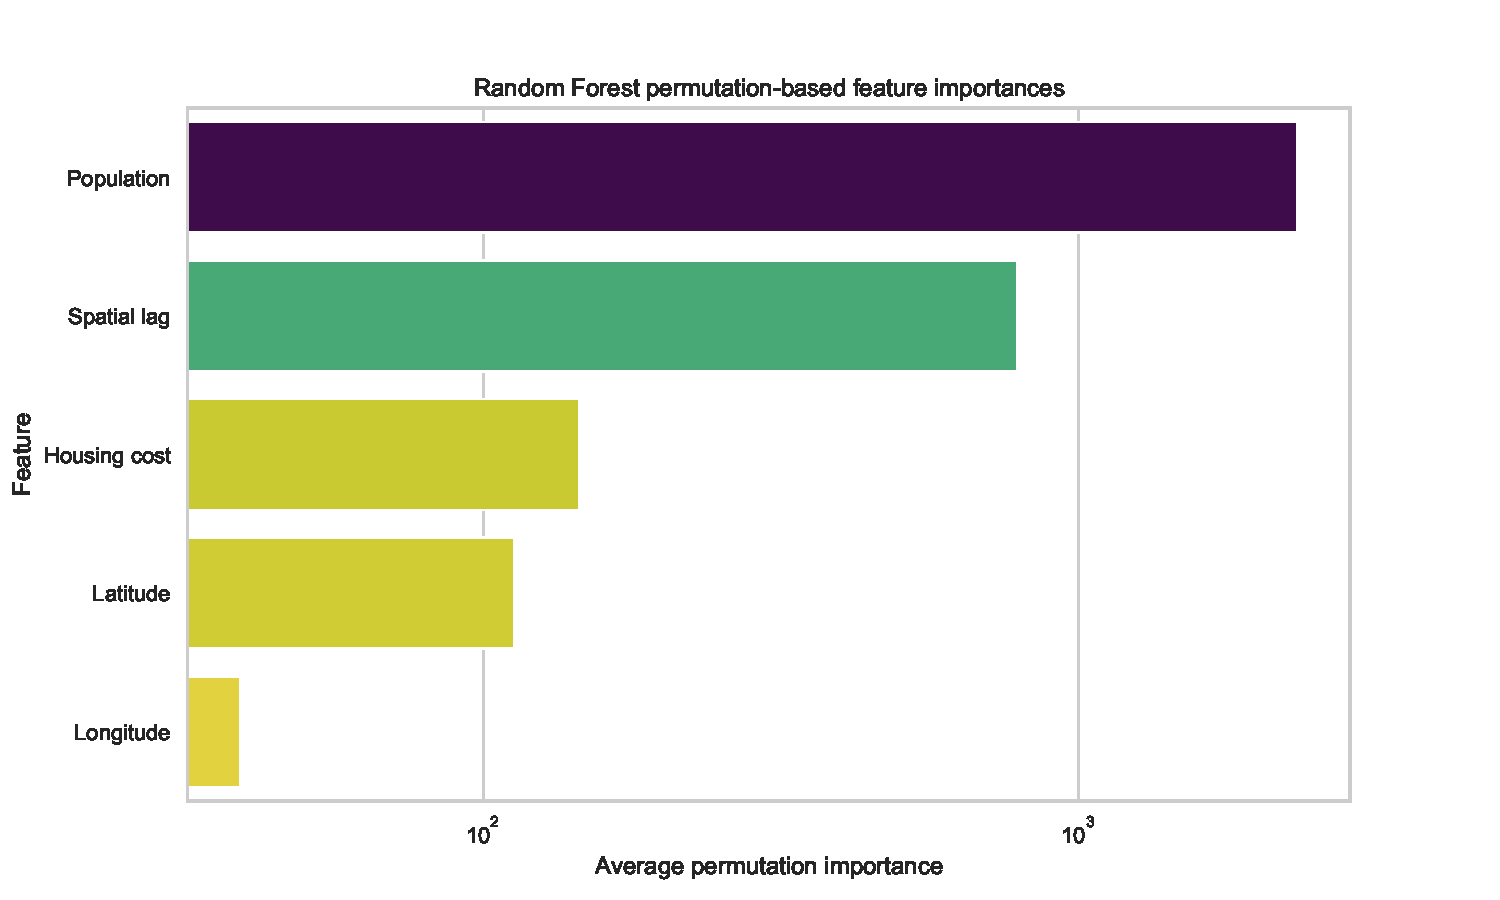
\includegraphics[width=0.5\linewidth]{figures/rf_feature_importance}
    \caption{
        \label{fig:feature_importance}
        Random Forest feature importances based on Gini impurity (left) and permutation importance (right). Both methods highlight population as the most dominant predictive feature.
    }
\end{figure}

We evaluated the model's performance across all 31 possible combinations of the five input features to select the most robust set (\autoref{fig:feature_combinations_rmse}). While the combination of all five features is not the single best performer, it is among the top tier, and the performance gains from excluding certain features are marginal. We therefore retained all five features in the final model to ensure it captures the broadest possible range of influencing factors.

The analysis in \autoref{fig:feature_combinations_rmse} offers a more complex picture of predictive factors. Contrary to what one might expect, the geographic coordinates (latitude and longitude) are surprisingly powerful. The model using only latitude and longitude is the third-best performer, suggesting that there are strong, spatially-defined patterns to homelessness that are not fully captured by our other variables. These could act as proxies for unmeasured factors like proximity to major urban centers, access to transportation networks, or historical social and economic conditions. Population remains a key variable, appearing in three of the top four models, but its predictive power is clearly enhanced by geographic context. Notably, neither spatial lag nor housing cost appear in the top-performing models, indicating their influence is secondary to these primary geographic and demographic factors.

\begin{figure}[htbp]
    \centering
    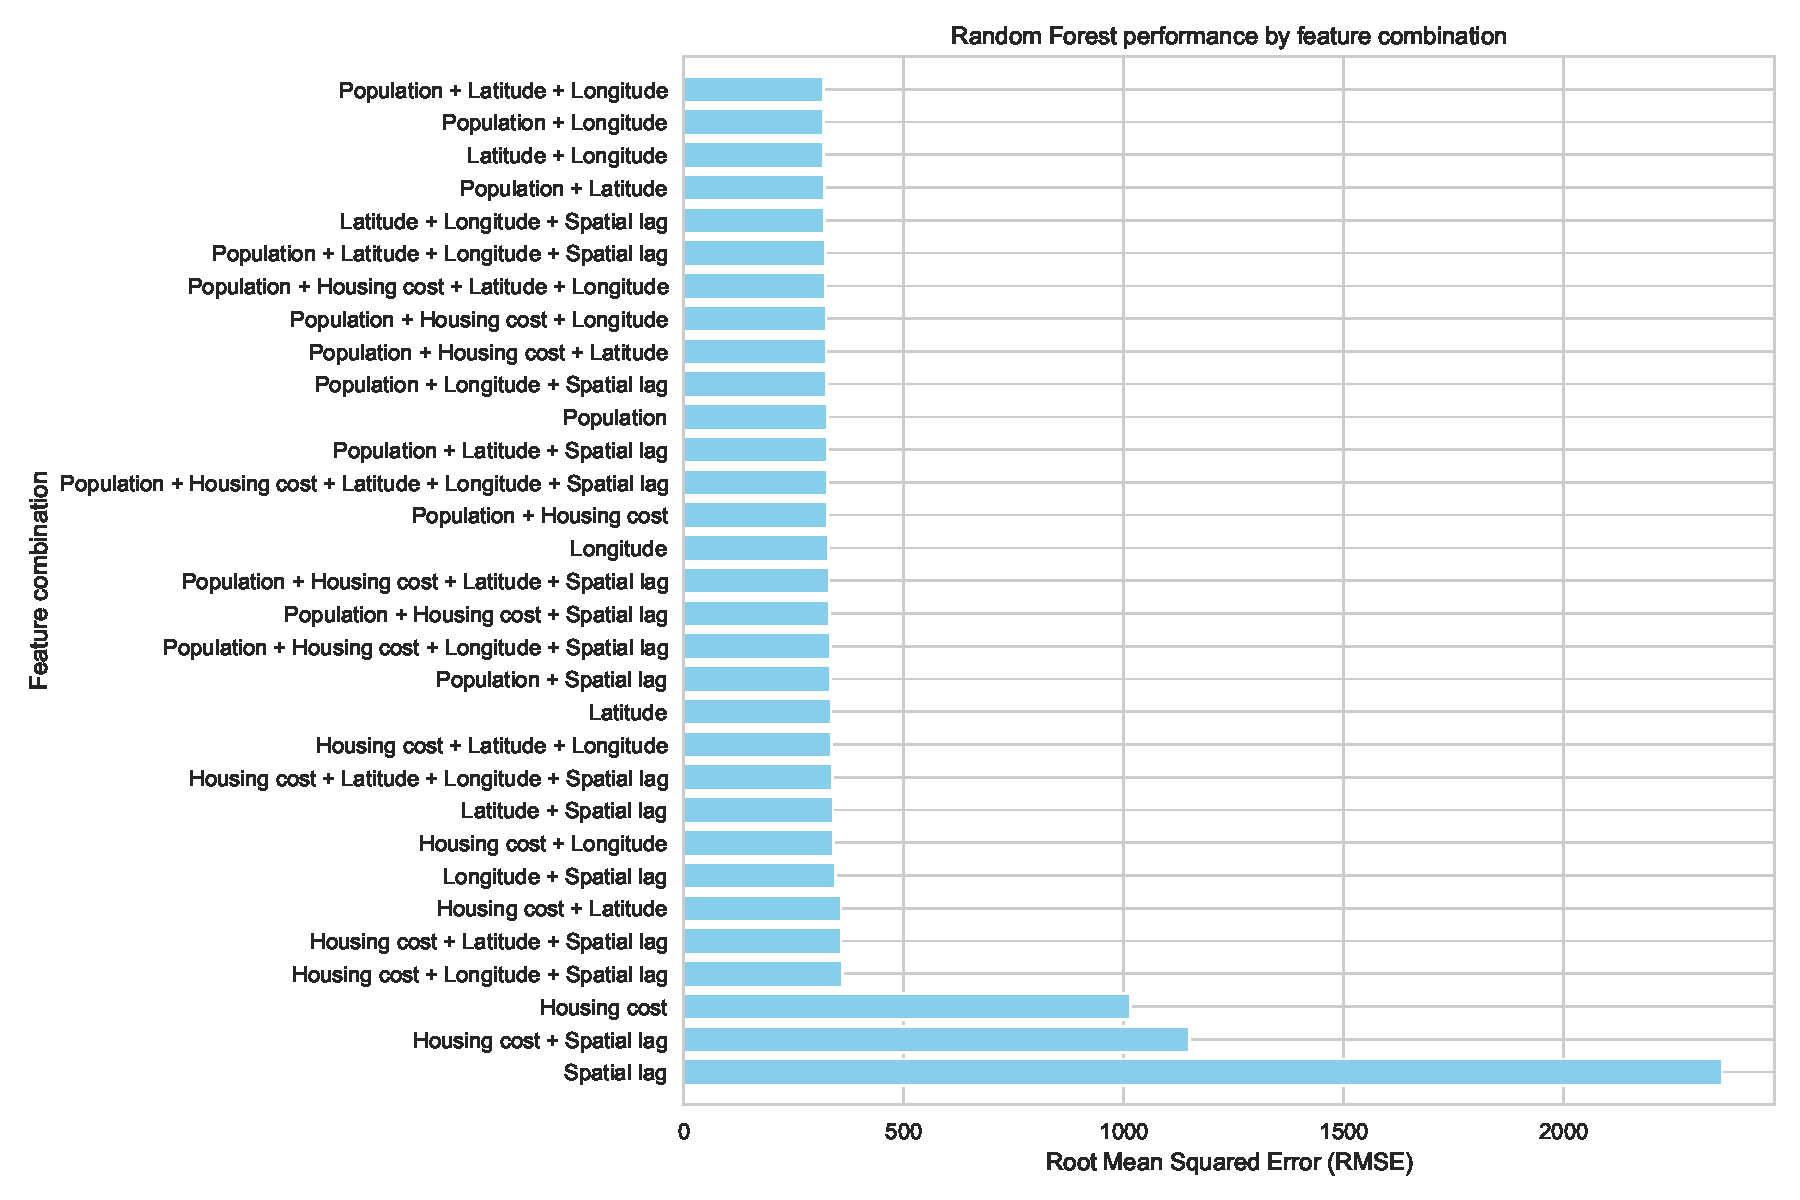
\includegraphics[width=\linewidth]{figures/RF_RMSE_Features}
    \caption{
        \label{fig:feature_combinations_rmse}
        Random Forest performance across all feature combinations.
    }
\end{figure}

% TODO: ANCOVA


\subsection{Assessing CoC effectiveness}

While the model confirms that population is the primary driver, our main goal is to look beyond external factors to assess CoC effectiveness. By using the model to predict homeless counts while holding population and housing costs constant at the state average, we can isolate and compare the underlying performance of each CoC. The results of this analysis are shown in \autoref{fig:maps:prediction} and~\ref{fig:predicted}.

\begin{figure}[htbp]
    \centering
    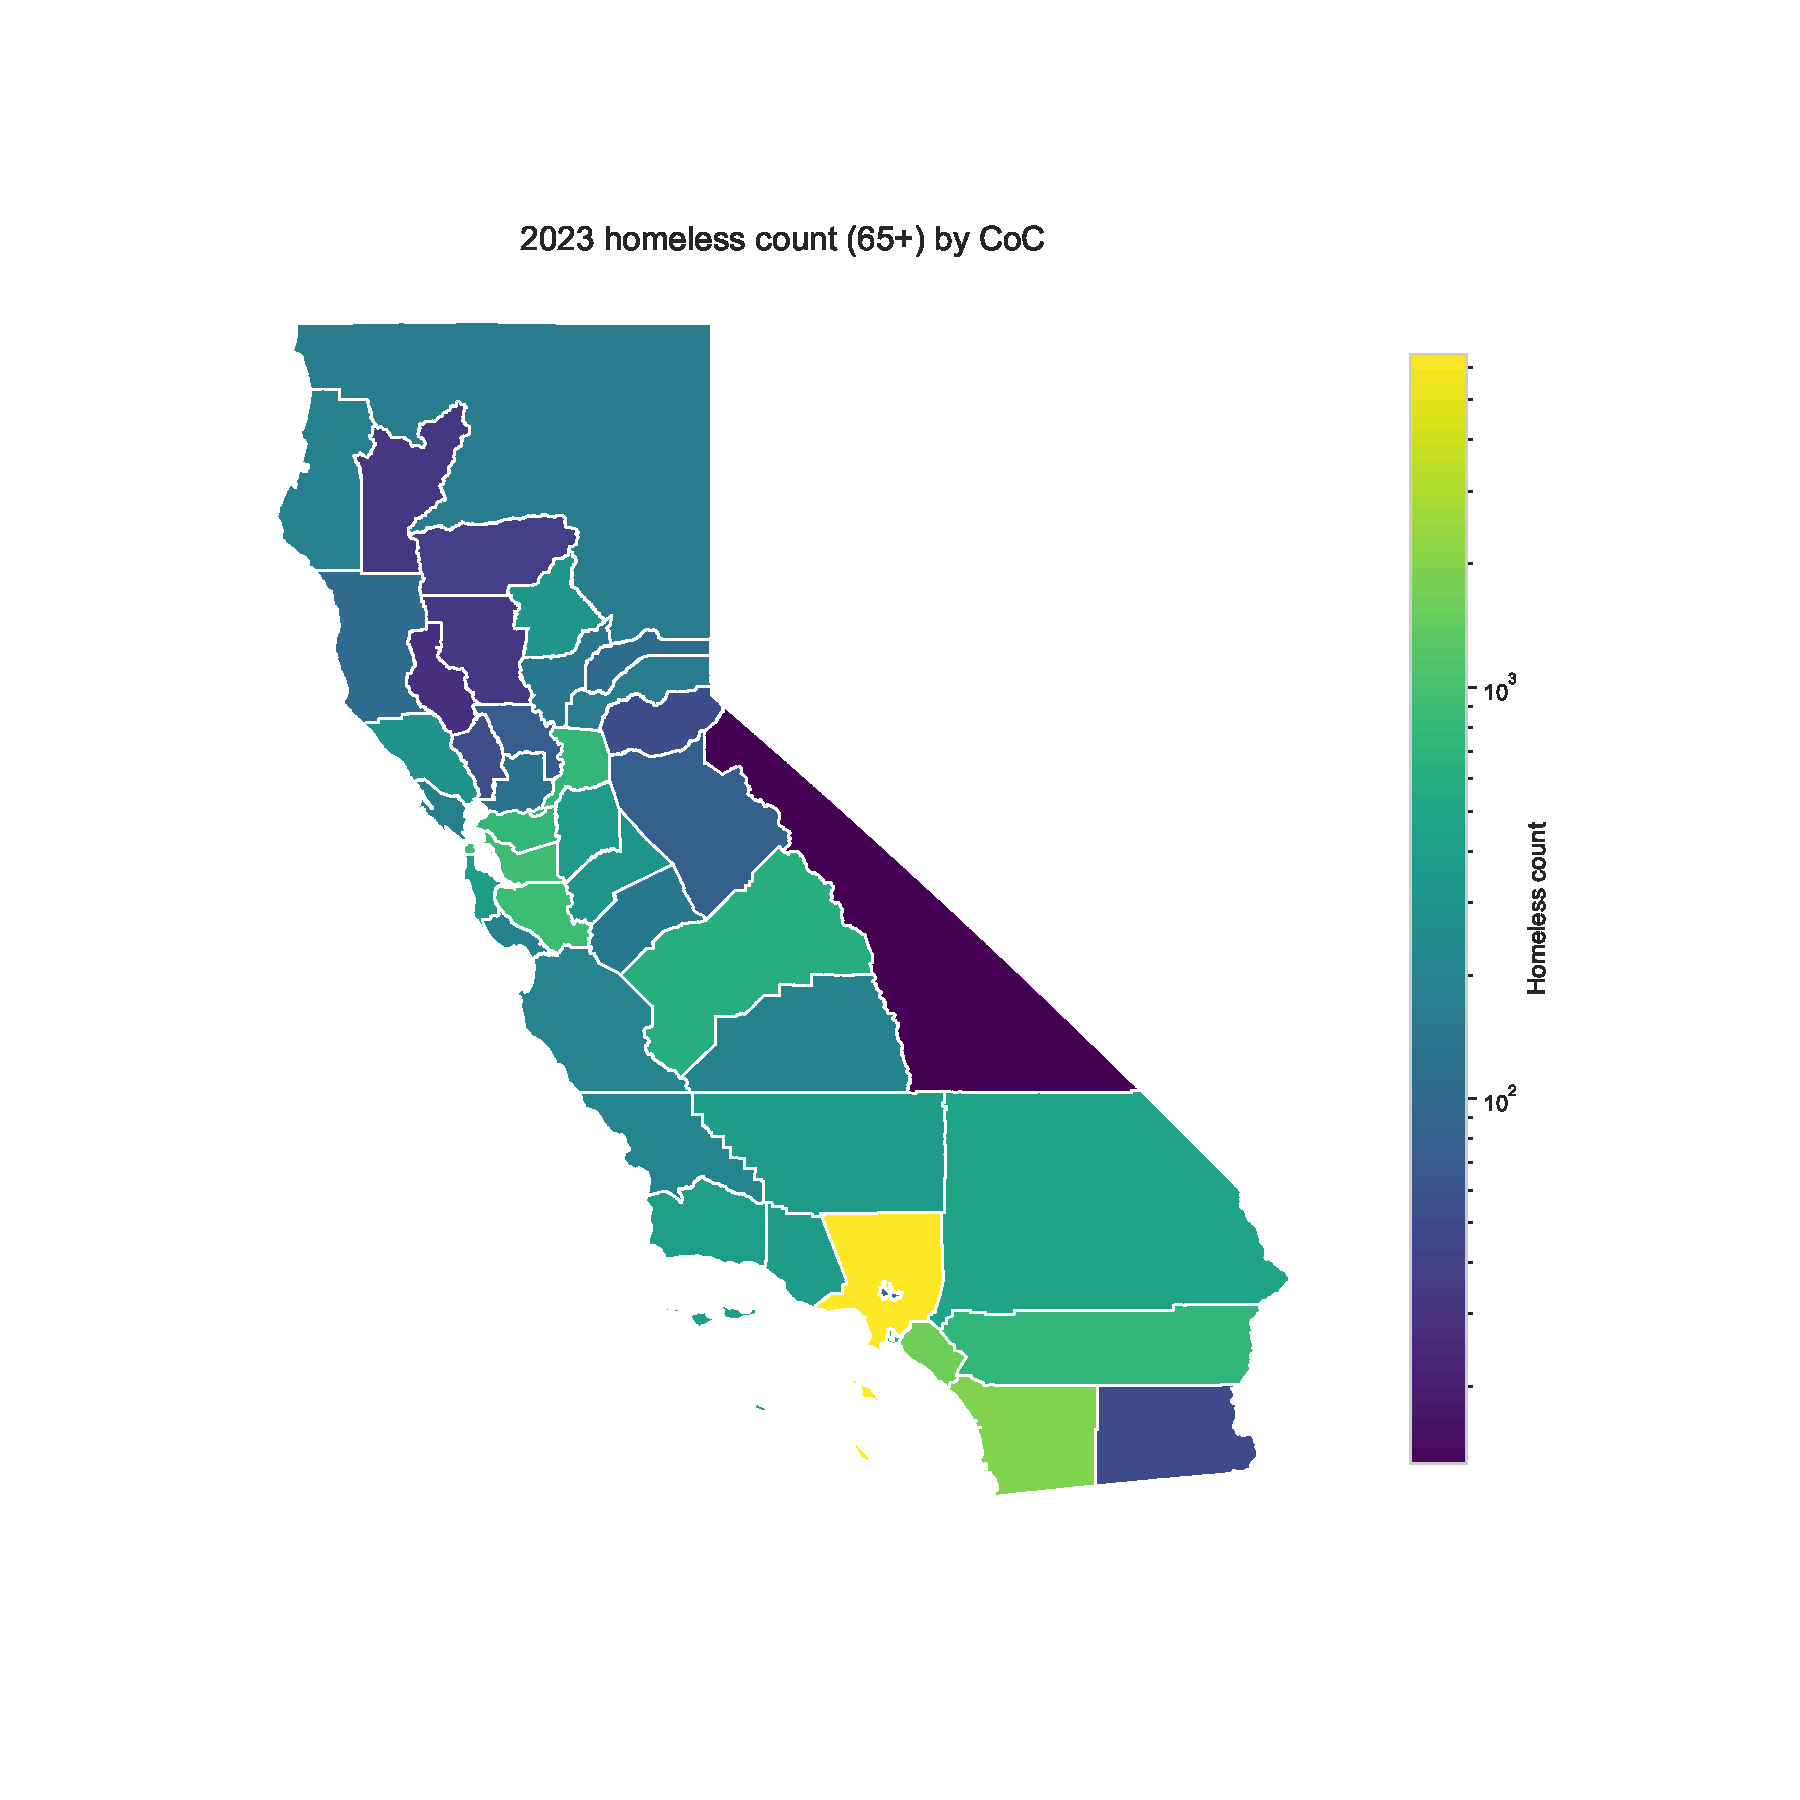
\includegraphics[width=0.5\linewidth, trim={1.5in 1.5in 1.5in 1in}, clip]{figures/maps/homeless_count}%
    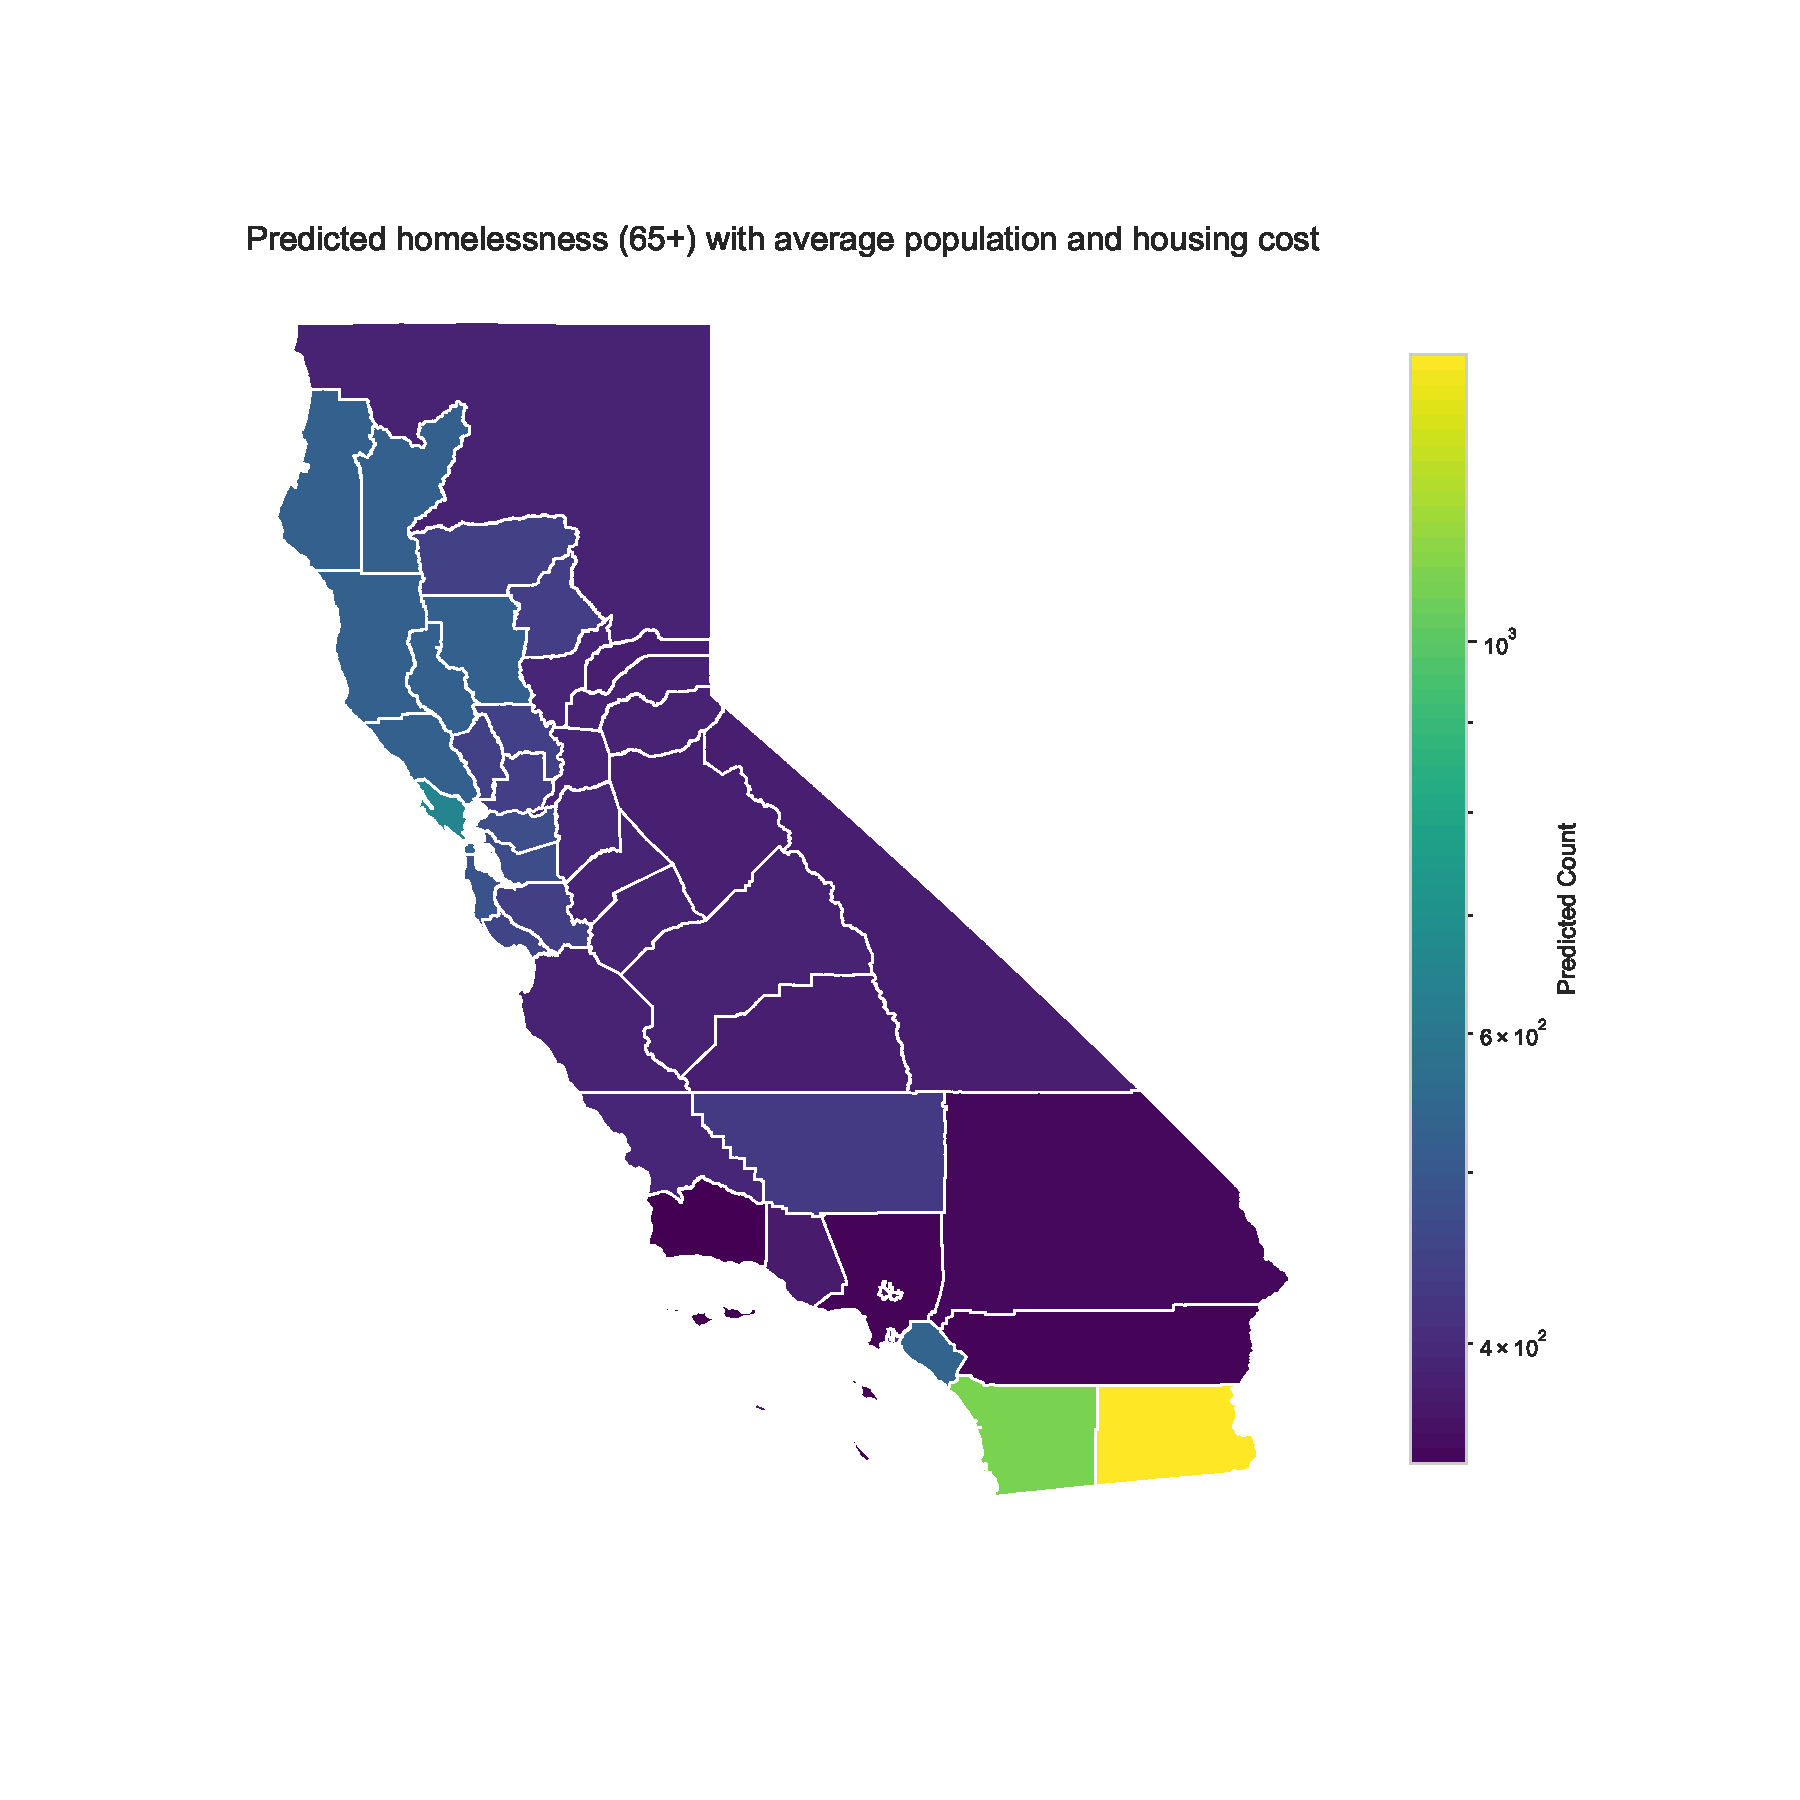
\includegraphics[width=0.5\linewidth, trim={1.5in 1.5in 1.5in 1in}, clip]{figures/maps/prediction_set}
    \caption{
        \label{fig:maps:prediction}
        65+ homeless population (left) and predicted 65+ homeless population when controlling for population and housing cost (right) in California CoCs in 2023 (log scale).
    }
\end{figure}


\begin{figure}[htbp]
    \centering
    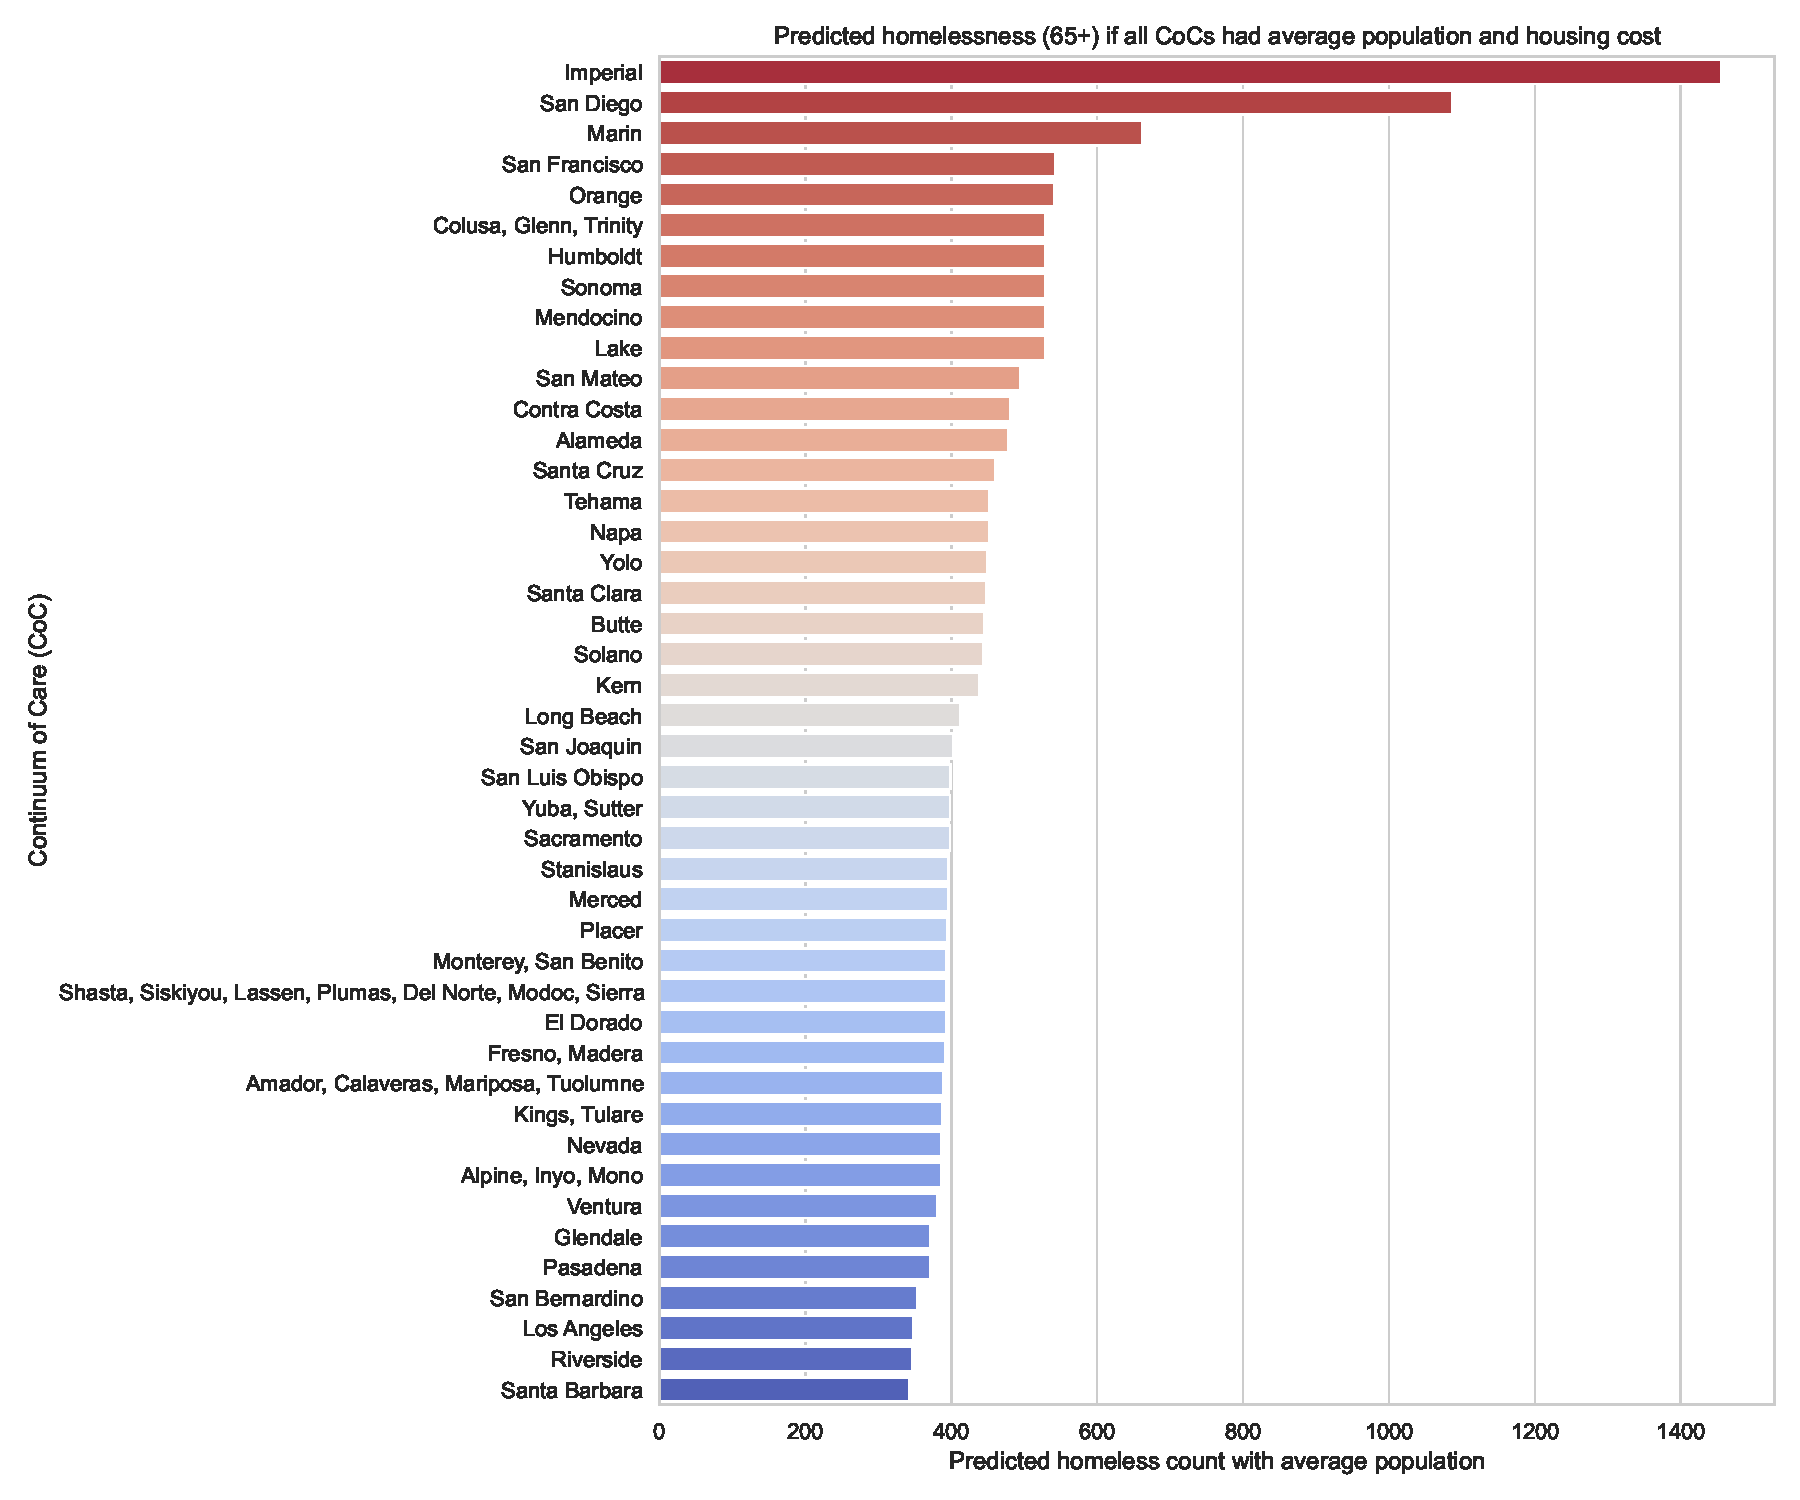
\includegraphics[width=\linewidth]{figures/predicted_chart}
    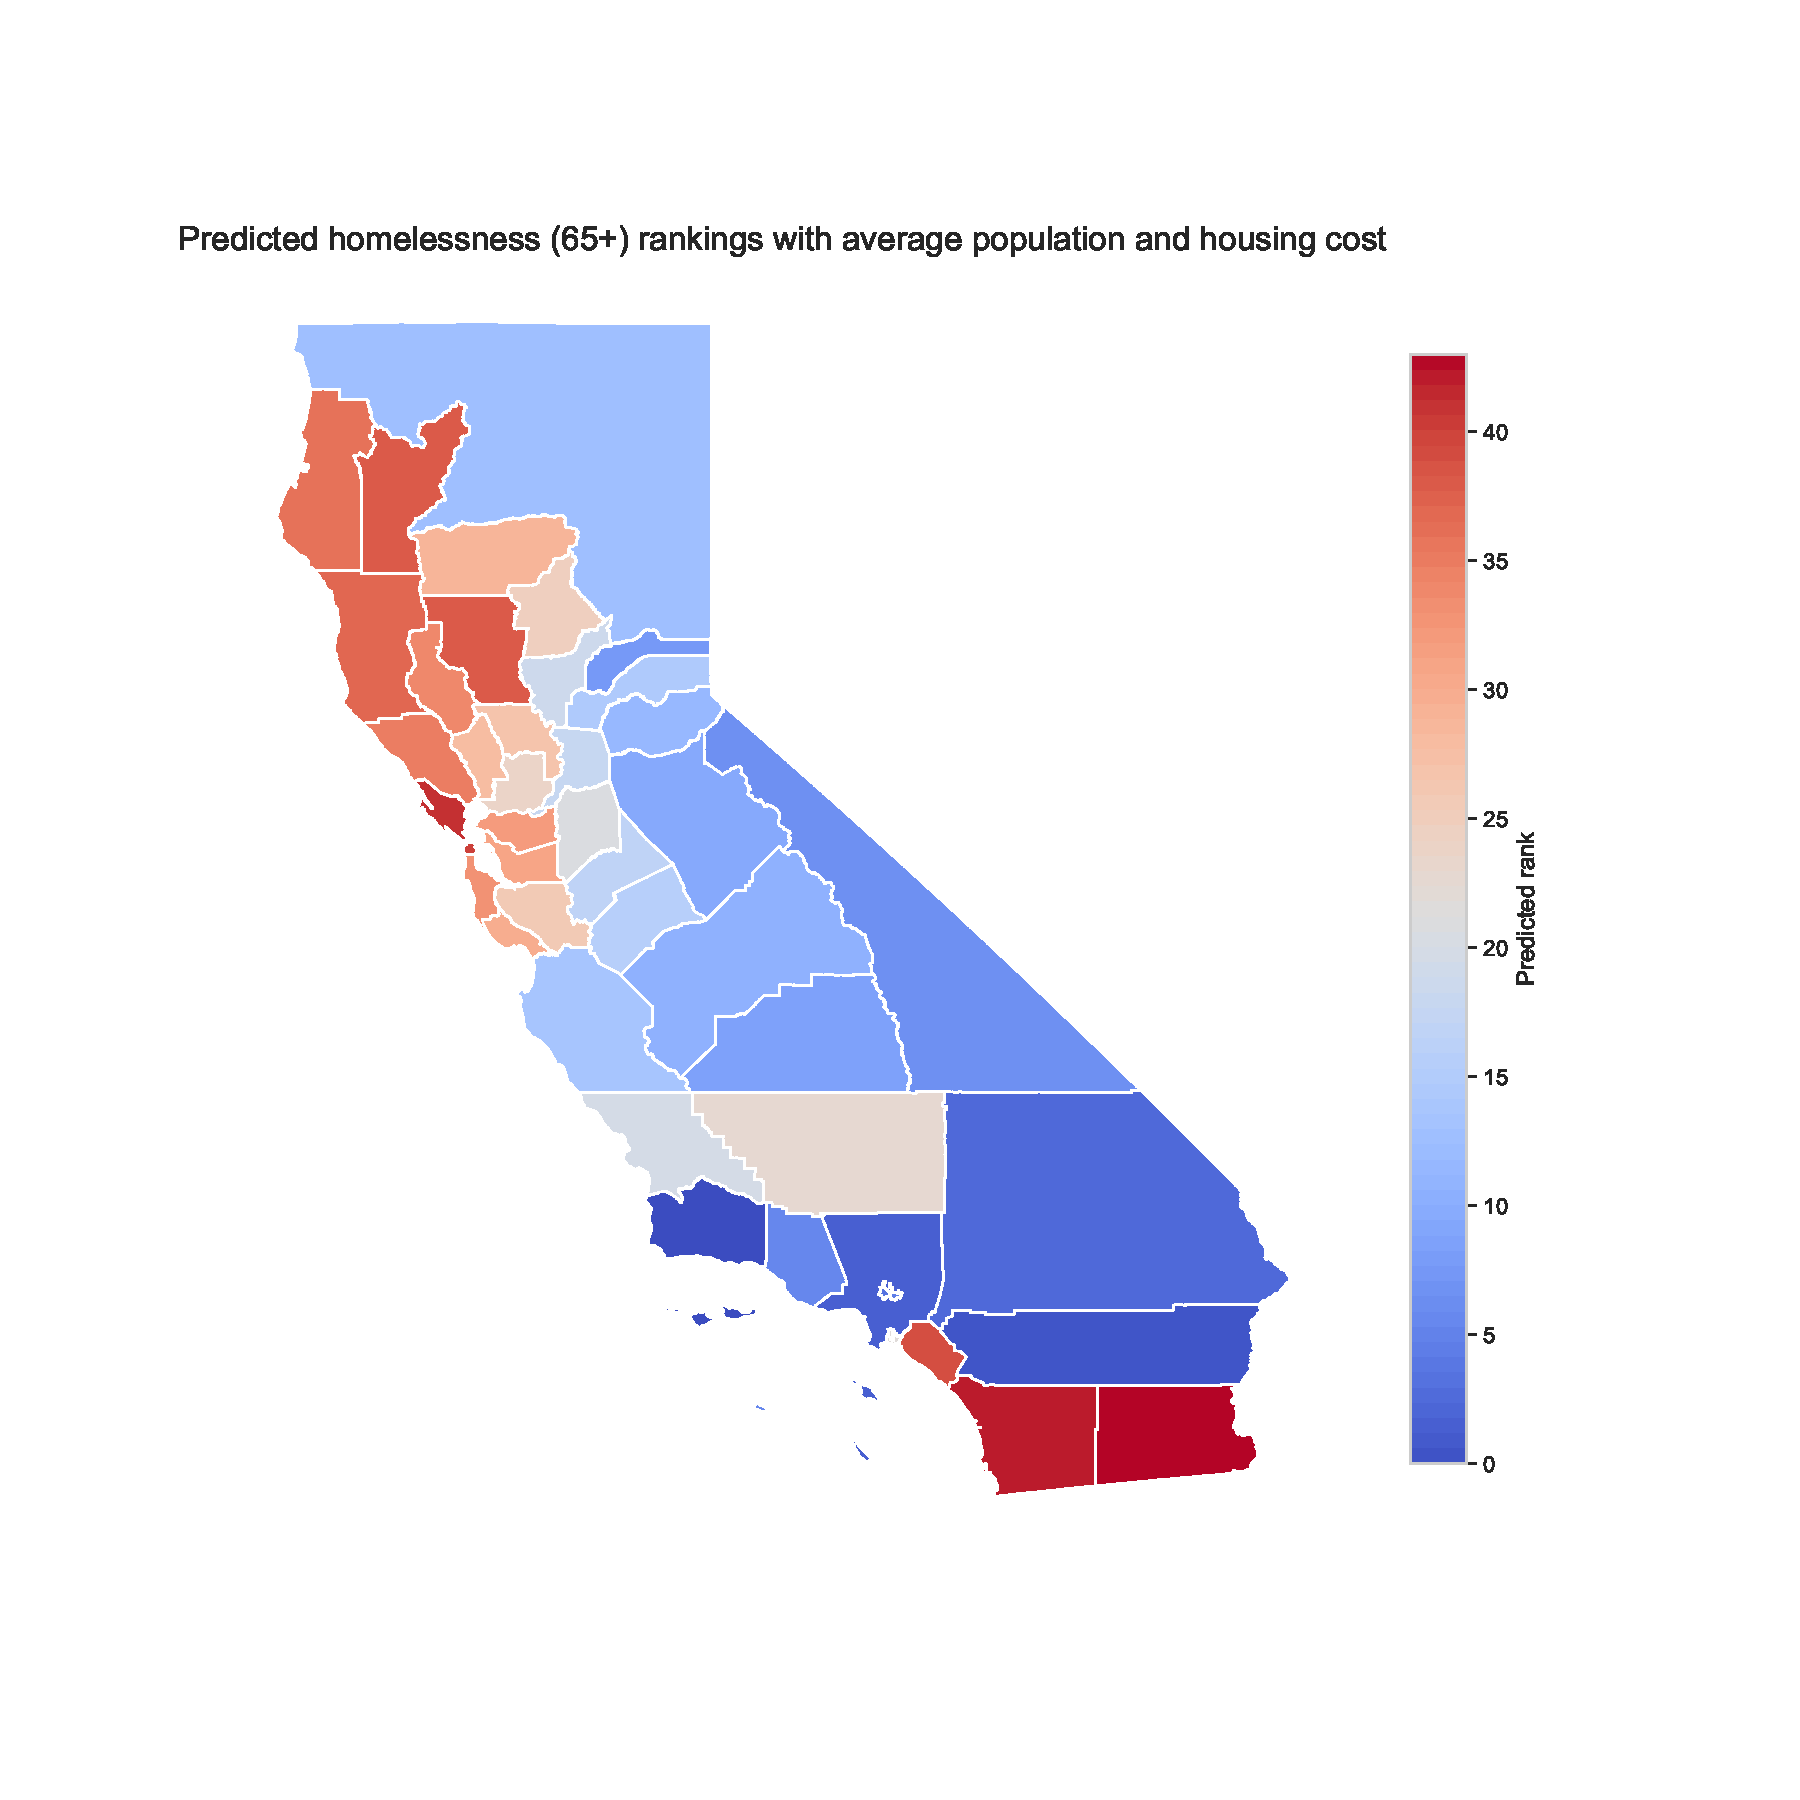
\includegraphics[width=0.6\linewidth, trim={1in 1.5in 1.5in 1in}, clip]{figures/maps/prediction_ranks}
    \caption{
        \label{fig:predicted}
        Predicted homelessness counts per CoC if all CoCs had average population and housing costs. This normalized view highlights CoCs that are performing better (e.g., Los Angeles) or worse (e.g., San Diego, Marin) than expected.
    }
\end{figure}

This normalized comparison reveals a landscape of CoC performance that is markedly different from the one suggested by the raw homeless counts. Two main regions of concern emerge, where homelessness is predicted to be higher than expected. The most prominent is in the southern part of the state, centered on Imperial and San Diego counties. A secondary area of concern appears in the northern coastal region, including Marin, Sonoma, and Humboldt counties. This suggests that factors unique to these CoCs---potentially related to local economic conditions, resource allocation, or specific policies---may be contributing to poorer outcomes. These areas warrant closer, qualitative investigation to understand the specific challenges they face.

Perhaps the most compelling finding is the emergence of CoCs that are performing significantly better than expected. This group includes large county-level CoCs like Los Angeles, Riverside, and San Bernardino, as well as smaller city-level CoCs within Los Angeles County: Glendale, Pasadena, and Long Beach. These CoCs have some of the highest absolute numbers of homeless seniors, but our model suggests they are managing the crisis more effectively than their large populations and high housing costs would predict. When these factors are neutralized, these CoCs show some of the lowest predicted homeless counts in the state. This finding does not diminish the scale of the crisis in these regions, but it reframes the narrative. It suggests that, relative to the scale of their challenge, the strategies employed by these large urban CoCs may be comparatively effective.

This analysis provides a new lens for policymakers and support organizations. Instead of focusing solely on the CoCs with the highest raw numbers, it may be more impactful to direct support and technical assistance to the regions of concern identified by the model---areas that appear to be underperforming regardless of their size. At the same time, the CoCs performing better than expected may offer valuable lessons and scalable strategies that could be adapted for use in other CoCs across the state.

\section{Acknowledgments}

This work was made possible through the dedicated efforts and support of Real Good AI, a 501(c)(3) nonprofit committed to advancing the world through the power of AI for good, providing AI support to organizations that strive for a brighter future~\cite{realgoodai}.

%\clearpage
\bibliographystyle{plainnat}
\bibliography{references}

\end{document}
